% License: LaTeX Project Public License 1.3c
% file dcmi.tex
% This is the LaTeX source for the instructions to authors using
% the LaTeX2e package 'dcmi.sty' for contributions to
% the DCMI Conferences.

\documentclass[11pt,a4paper]{article}

% if you need to pass options to natbib, use, e.g.:
%     \PassOptionsToPackage{numbers, compress}{natbib}
% before loading dcmi

% load package
\usepackage{dcmi}

\usepackage[utf8]{inputenc} % allow utf-8 input
\usepackage[T1]{fontenc}    % use 8-bit T1 fonts
\usepackage{hyperref}       % hyperlinks
\usepackage{url}            % simple URL typesetting
\usepackage{booktabs}       % professional-quality tables
\usepackage{amsfonts}       % blackboard math symbols
\usepackage{nicefrac}       % compact symbols for 1/2, etc.
\usepackage{microtype}      % microtypography
\usepackage[pdftex]{graphicx}       % figures
\usepackage{sectsty}		% section titles

\usepackage[strings]{underscore}
\usepackage[backend=biber, style=apa]{biblatex}
\usepackage[american]{babel}
\usepackage{csquotes}
\DeclareLanguageMapping{american}{american-apa}
% Edit and uncomment below line to load your bibliography
% \addbibresource{reference.bib} %Imports bibliography file

% section title font settings
\allsectionsfont{\sffamily}
\sectionfont{\sffamily\fontsize{12}{15}\selectfont}
\subsectionfont{\sffamily\fontsize{11}{14}\selectfont}
\subsubsectionfont{\sffamily\fontsize{10}{14}\selectfont\itshape}

\title{\LaTeX{} Template for the International Conference on Dublin Core and Metadata Applications}

% The \author macro works with any number of authors. There are two commands
% used to separate the names and addresses of multiple authors: \And and \AND.
%
% Using \And between authors leaves it to LaTeX to determine where to break the
% lines. Using \AND forces a line break at that point. So, if LaTeX puts 3 of 4
% authors names on the first line, and the last on the second line, try using
% \AND instead of \And before the third author name.

\author{%
  First Author\thanks{Use footnote for providing further information
    about author (webpage, alternative address)---\emph{not} for acknowledging
    funding agencies.} \\
  Department \\
  Affiliation\\
  Country \\
  \texttt{author@inst.tld} \\
  % examples of more authors
  \And
  Coauthor \\
  Department \\
  Affiliation \\
  Country \\
  \texttt{coauthor@inst.tld} \\
  \And
  Coauthor \\
  Department \\
  Affiliation \\
  Country \\
  \texttt{coauthor@another-inst.tld} \\
  % \AND
  % Coauthor \\
  % Affiliation \\
  % Address \\
  % \texttt{email} \\
  % \And
  % Coauthor \\
  % Affiliation \\
  % Address \\
  % \texttt{email} \\
}

\begin{document}

\maketitle

\begin{abstract}
  The abstract text is in Times New Roman, 11 point and should be no more than 250 words in length. The abstract must be limited to one paragraph. Keywords must be entered using lower-case letters except for proper nouns which should have the first letter of each word capitalized.  Each keyword or keyword phrase should be separated by a semicolon (e.g., “metadata; evaluation; visual graphic analysis”).
\end{abstract}

\keywords{metadata; evaluation; visual graphic analysis}

% Start footnote numbering from 1, if \thanks command is used
\setcounter{footnote}{0}

\section{Submission of papers to DCMI 2023}

DCMI requires electronic submissions.  The electronic submission site is
\begin{center}
  \url{https://easychair.org/conferences/?conf=dcmi2023}
\end{center}

Please read the instructions below carefully and follow them faithfully.

\subsection{Style}

Papers to be submitted to DCMI 2023 must be prepared according to the
instructions presented here.

Authors are required to use the DCMI \LaTeX{} style files obtainable at the
DCMI website as indicated below. Tweaking the style files may be grounds for
rejection.

\subsection{Retrieval of style files}

The style files for DCMI 2023 are available on
the World Wide Web at
\begin{center}
  \url{https://github.com/dcmi/dcpapers-templates}
\end{center}
The file \verb+dcmi_template.pdf+ contains these instructions and illustrates the
various formatting requirements your DCMI paper must satisfy.

The file \verb+dcmi_template.tex+ may be used as a ``shell'' for writing your
paper. All you have to do is replace the author, title, abstract, and text of
the paper with your own.

The formatting instructions contained in these style files are summarized in
Sections \ref{gen_inst}, \ref{headings}, and \ref{others} below.

\section{General formatting instructions}
\label{gen_inst}

Times New Roman is the preferred typeface throughout, and will be selected for you by default.
Paragraphs are separated by \nicefrac{1}{2}~line space (5.5 points), with no
indentation.

The paper title should be 17~point, initial caps/lower case, bold, centered.
Allow an extra \nicefrac{1}{4}~inch space above and
below the title. All pages should start at 1~inch (6~picas) from the
top of the page.

For the final version, authors' names are set in boldface, and each name is
centered above the corresponding address. The lead author's name is to be listed
first (left-most), and the co-authors' names (if different address) are set to
follow. If there is only one co-author, list both author and co-author side by
side.

Please pay special attention to the instructions in Section \ref{others}
regarding figures, tables, acknowledgments, and references.

\section{Headings: first level}
\label{headings}

All headings should be lower case (except for first word and proper nouns),
flush left, and bold.

First-level headings should be in 12-point type.

\subsection{Headings: second level}

Second-level headings should be in 11-point type.

\subsubsection{Headings: third level}

Third-level headings should be in 11-point type and Italics.


\section{Citations, figures, tables, references}
\label{others}

These instructions apply to everyone.

\subsection{Citations within the text}

The DCMI Proceedings use a small subset of modified rules from the American Psychological Association (APA) Publication Manual.  All in-text references take the form of parentheticals.  The following examples of in-text citation are to works in the Reference section below.

\begin{quote}
“According to Hillmann (2006) and Heery (2004, pp. 258-59)…”

“The first publication of the Dublin Core Element Set was early in the history of the Initiative (DCMI, 1998)…”

“…have resulted in new conceptions of a digital library (Lagoze et al., 2005)…”
\end{quote}


In the paper’s reference section, the names of authors must be spelled out.  With multiple authors, only the first named author begins with the family name followed by a comma and the first name.  Any remaining authors are listed with given name first followed by family name.

The APA Publication Manual should be consulted for answers to questions of style not addressed in these instructions.

The \verb+biblatex+ package will be loaded for you by default. The documentation for \verb+biblatex+ may be found at
\begin{center}
\url{https://ctan.org/pkg/biblatex}
\end{center}
Of note is the command \verb+\citet+, which produces citations appropriate for
use in inline text.  For example,
\begin{verbatim}
   \citet{hasselmo} investigated\dots
\end{verbatim}
produces
\begin{quote}
  Hasselmo, et al.\ (1995) investigated\dots
\end{quote}

If you wish to load the \verb+natbib+ package with options, you may add the
following before loading the \verb+dc2002+ package:
\begin{verbatim}
   \PassOptionsToPackage{options}{natbib}
\end{verbatim}

You can optionally use \verb+biblatex+ package instead of \verb+natbib+.

\subsection{Footnotes}

Footnotes should be used sparingly.  If you do require a footnote, indicate
footnotes with a number\footnote{Sample of the first footnote.} in the
text. Place the footnotes at the bottom of the page on which they appear.
Precede the footnote with a horizontal rule of 2~inches (12~picas).

Note that footnotes are properly typeset \emph{after} punctuation
marks.\footnote{As in this example.}

\subsection{Figures}

\begin{figure}
  \centering
  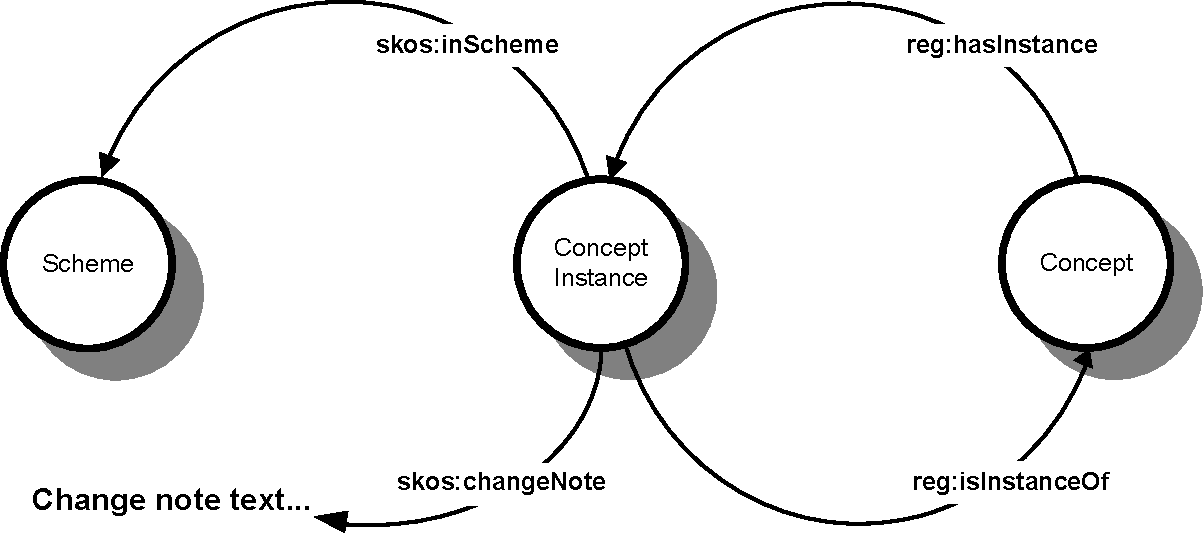
\includegraphics[width=0.6\linewidth]{figure.pdf}
  \caption{Sample figure caption.}
\end{figure}

All artwork must be neat, clean, and legible. Lines should be dark enough for
purposes of reproduction. The figure number and caption always appear after the
figure. Place one line space before the figure caption and one line space after
the figure. The figure caption should be lower case (except for first word and
proper nouns); figures are numbered consecutively.

You may use color figures.  However, it is best for the figure captions and the
paper body to be legible if the paper is printed in either black/white or in
color.

\subsection{Tables}

All tables must be centered, neat, clean and legible.  The table number and
title always appear before the table.  See Table~\ref{sample-table}.

Place one line space before the table title, one line space after the
table title, and one line space after the table. The table title must
be lower case (except for first word and proper nouns); tables are
numbered consecutively.

Note that publication-quality tables \emph{do not contain vertical rules.} We
strongly suggest the use of the \verb+booktabs+ package, which allows for
typesetting high-quality, professional tables:
\begin{center}
  \url{https://www.ctan.org/pkg/booktabs}
\end{center}
This package was used to typeset Table~\ref{sample-table}.

\begin{table}
  \caption{Sample table title}
  \label{sample-table}
  \centering
  \begin{tabular}{lll}
    \toprule
    \multicolumn{2}{c}{Part}                   \\
    \cmidrule(r){1-2}
    Name     & Description     & Size ($\mu$m) \\
    \midrule
    Dendrite & Input terminal  & $\sim$100     \\
    Axon     & Output terminal & $\sim$10      \\
    Soma     & Cell body       & up to $10^6$  \\
    \bottomrule
  \end{tabular}
\end{table}

\section{Final instructions}

Do not change any aspects of the formatting parameters in the style files.  In
particular, do not modify the width or length of the rectangle the text should
fit into, and do not change font sizes (except perhaps in the
\textbf{References} section; see below). Please note that pages should be
numbered.

\section{Preparing PDF files}

Please prepare submission files with paper size ``A4,'' and not, for
example, ``US Letter.''

Fonts were the main cause of problems in the past years. Your PDF file must only
contain Type 1 or Embedded TrueType fonts. Here are a few instructions to
achieve this.

\begin{itemize}

\item You should directly generate PDF files using \verb+pdflatex+.

\item You can check which fonts a PDF files uses.  In Acrobat Reader, select the
  menu Files$>$Document Properties$>$Fonts and select Show All Fonts. You can
  also use the program \verb+pdffonts+ which comes with \verb+xpdf+ and is
  available out-of-the-box on most Linux machines.

\item The IEEE has recommendations for generating PDF files whose fonts are also
  acceptable for DC. Please see
  \url{http://www.emfield.org/icuwb2010/downloads/IEEE-PDF-SpecV32.pdf}

\item \verb+xfig+ "patterned" shapes are implemented with bitmap fonts.  Use
  "solid" shapes instead.

\item The \verb+\bbold+ package almost always uses bitmap fonts.  You should use
  the equivalent AMS Fonts:
\begin{verbatim}
   \usepackage{amsfonts}
\end{verbatim}
followed by, e.g., \verb+\mathbb{R}+, \verb+\mathbb{N}+, or \verb+\mathbb{C}+
for $\mathbb{R}$, $\mathbb{N}$ or $\mathbb{C}$.  You can also use the following
workaround for reals, natural and complex:
\begin{verbatim}
   \newcommand{\RR}{I\!\!R} %real numbers
   \newcommand{\Nat}{I\!\!N} %natural numbers
   \newcommand{\CC}{I\!\!\!\!C} %complex numbers
\end{verbatim}
Note that \verb+amsfonts+ is automatically loaded by the \verb+amssymb+ package.

\end{itemize}

If your file contains type 3 fonts or non embedded TrueType fonts, we will ask
you to fix it.

\subsection{Margins in \LaTeX{}}

Most of the margin problems come from figures positioned by hand using
\verb+\special+ or other commands. We suggest using the command
\verb+\includegraphics+ from the \verb+graphicx+ package. Always specify the
figure width as a multiple of the line width as in the example below:
\begin{verbatim}
   \usepackage[pdftex]{graphicx} ...
   \includegraphics[width=0.8\linewidth]{myfile.pdf}
\end{verbatim}
See Section 4.4 in the graphics bundle documentation
(\url{http://mirrors.ctan.org/macros/latex/required/graphics/grfguide.pdf})

A number of width problems arise when \LaTeX{} cannot properly hyphenate a
line. Please give LaTeX hyphenation hints using the \verb+\-+ command when
necessary.


\begin{ack}
Use unnumbered first level headings for the acknowledgments. All acknowledgments
go at the end of the paper before the list of references.

You can use the \texttt{ack} environment provided in the style file to automatically hide this section in the anonymized submission.
\end{ack}

\section*{References}

References follow the acknowledgments. It is permissible to reduce the font size to \verb+small+ (9 point) when listing the references. You can use \verb+biblatex+ or  \verb+natbib+ to generate your references list.

{\bf Note that the Reference section does not count towards the number of pages of content that is allowed.}
\medskip

\small


\hangindent=0.7cm DCMI. (1998).  Dublin Core Metadata Element Set, version 1.0: Reference description.  Retrieved January 10, 2007, from \url{http://www.dublincore.org/documents/1998/09/dces/}.

\hangindent=0.7cm Heery, Rachel.  (2004). Metadata futures: Steps toward semantic interoperability. In Diane I. Hillmann \& Elaine L. Westbrooks (Eds.), {\it Metadata in practice}  (pp. {\bf 257-271
}).  Chicago: American Library Association.

\hangindent=0.7cm Hillmann, Diane. I., Stuart A. Sutton, Jon Phipps, and Ryan J. Laundry.\ (2006). A metadata registry from vocabularies up: The NSDL registry project.  {\it Proceedings of the International Conference on Dublin Core and Metadata Applications}, 2006, 65-75.

\hangindent=0.7cm Lagoze, Carl, Dean Krafft, Sandy Payette, and Susan Jesuroga. (2005, November). What is a digital library anyway, anymore? Beyond search and access in the NSDL.  D-Lib Magazine, 11(11).  Retrieved, January 10, 2007, from \url{http://www.dlib.org/dlib/november05/lagoze/11lagoze.html}



\end{document}